% University of Michigan Dissertation LaTeX Template for 2019 -- 2020
% Created by John Meluso and Shreyas Kousik
% 9 Jul 2020

% Use the University of Michigan thesis class.
\documentclass[thesis]{thesis-umich}
%%% Packages included in thesis-umich class
%\RequirePackage[margin=1in,footskip=8pt,headsep=0.4cm,headheight=\baselineskip]{geometry}
%\RequirePackage{amsmath}
%\RequirePackage{amsfonts}
%\RequirePackage{amssymb}
%\RequirePackage{graphicx}
%\RequirePackage{subcaption}
%\RequirePackage{times}
%\RequirePackage{natbib}
%\RequirePackage{verbatim}
%\RequirePackage{upquote}
%\RequirePackage{textcomp}
%\RequirePackage{setspace}
%\RequirePackage{ifthen}
%\RequirePackage{soul}
%\RequirePackage{float}
%\RequirePackage[printonlyused]{acronym}
%\RequirePackage{makeidx}
%\RequirePackage{fancyhdr}
%\RequirePackage{multicol}

% Include your packages here by including a \usepackage{<package_name>} command.
\usepackage{blindtext} % Example package which populates the ever-popular lorem ipsum text.

% If you are using the alpha bibliography style, keep these next three lines in your preamble, so that the references are left-aligned; or, you can comment it out and see what happens
\makeatletter
\renewcommand{\@biblabel}[1]{[#1]\hfill}
\makeatother

% Title of the thesis
\title{Your Dissertation Title}

% Author name
\author{Your M. Name}

% Department
\department{Field of Degree (e.g. ``Psychology'')}

% Year of completion
\year=2020

% Author email
\email{youremail@umich.edu}

% Author ORCID iD
\orcid{0000-0000-0000-0000}

% Frontispiece
\frontispiece{
\includegraphics[width=4in]{front_materials/frontispiece.png}}

% Default style for front pages
\frontpagestyle{7} % 7 is preferred by Rackham, but should be set individually for each front page

% Dedication (the input [7] determines the style -- 7 is Rackham's preferred style)
% \hidededication{%
\dedication[7]{Put your dedication text here.}

% Acknowledgments (the input [7] determines the style -- 7 is Rackham's preferred style)
\acknowledgments[7]{Put your acknowledgements text here.}

% Preface
\preface[7]{\blindtext

\blindtext}

% Committee
\committee{ %
Professor First Name, Chair \\
Professor Second Name in Alphabetical Order \\
Professor Third Name in Alphabetical Order \\
Professor Fourth Name in Alphabetical Order
}

% Chair must be entered separately for formatting reasons.
\chair{Professor First Name}
%\cochair{Co-chair One \& Co-chair Two}

% Commands to hide or show lists of figures, tables, etc.
% To hide a list, change the word "show" in the command to "hide".
\showlistoftables
\showlistofprograms
\showlistofappendices
\showlistofacronyms


% Definition of any acronyms used.
% To add an acronym, add an \acro{}{} command on a new line within the \acronyms{} command. For \acro, field 1 is the acronym and field 2 is the corresponding expression. For example: \acro{TLA}{Three Letter Acronym}.
\acronyms{
    \acro{TLA}{Three Letter Acronym}
    \acro{SOA}{Some Other Acronym}
}

% Some abstract text
\abstract{
Put your abstract text here.
}
%\hideabstractpagenumber

%% DOCUMENT AREA
\begin{document}

\chapter{Introduction}
\label{chpt:introduction}

This is a dissertation template. Here is the introduction text. As with this chapter, add other chapters to the dissertation and cite them in the ``main.tex'' file.


\section{Example Section}
\label{sec:examplesec1}

This dissertation template combines the work of our fore-academics to build a format that works for all of those who use \LaTeX \cite{jefferson2019policing}. We sincerely hope you find it useful \cite{shannon1948mathematical}.

You can add acronyms in the text and front table! See the comments around the acronyms command for how to include them in the front table. The first time you use an acronym in the text, use the ``\textbackslash ac\{\}'' command like with this \ac{TLA} or \ac{SOA}. After you use them the first time, it'll just appear as the acronym (like this: \ac{TLA}).

\blindtext


\section{Example Tables}
\label{sec:examplesec2}

You can make a table as follows \cite{ong1997gilbert}. Use can cross-reference items by doing things like Chapter \ref{chpt:introduction}.

\blindtext

\begin{table}[ht]
    \begin{tabular}{l|l}
        \textbf{left column} & \textbf{right column} \\ \hline
        entry1 & entry2 \\
        entry3 & entry4
    \end{tabular}
    \caption{An example table with things in it. Take a look at https://www.latex-tables.com/ for a relatively-easy latex table generator. Other options include https://truben.no/table/old/ and https://www.tablesgenerator.com/, but you'll find others online, too!}
    \label{tab:my-table}
\end{table}

\blindtext


\section{Example Figure}
\label{sec:examplesec3}

Check out Figure \ref{fig:the_big_house}. \blindtext

\begin{figure}
    \centering
    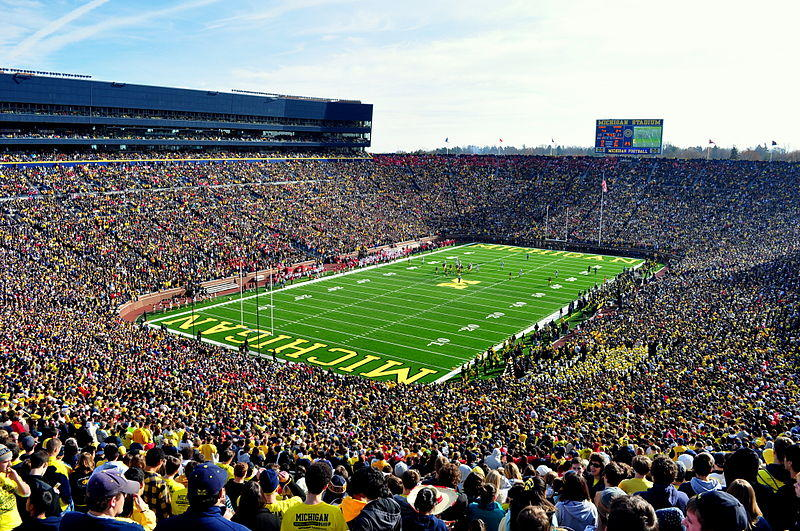
\includegraphics{chapters/figures/the_big_house.jpeg}
    \caption{The Big House, taken from Michigan Radio's article about it \cite{the_big_house}}
    \label{fig:the_big_house}
\end{figure}

\blindtext[3]
% Place your additional chapters here using the \input{} command
\chapter{Conclusion}
\label{chpt:conclusion}

Check out the Big House in another figure, Figure \ref{fig:the_big_house}. \blindtext

\begin{figure}
    \centering
    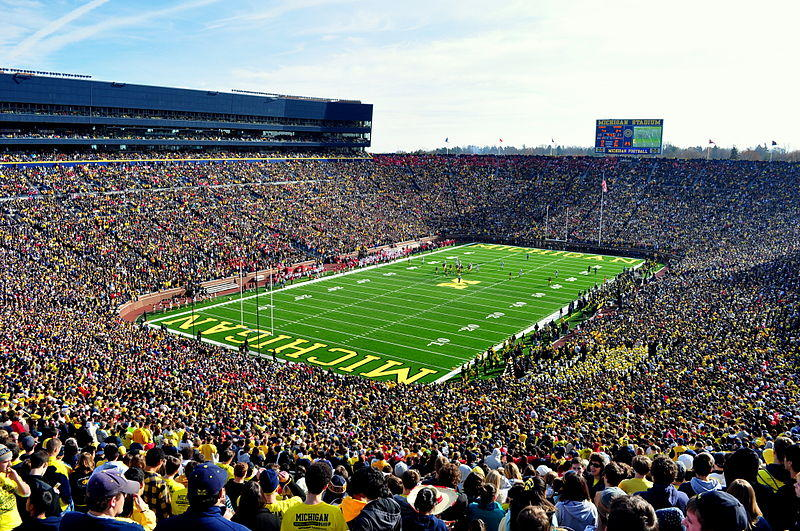
\includegraphics{chapters/figures/the_big_house.jpeg}
    \caption{The Big House (again!!), taken from Michigan Radio's article about it \cite{the_big_house}}
    \label{fig:the_big_house_2}
\end{figure}

% Appendices
\appendix
\chapter{Example Appendix 01}
\label{chpt:appendix_01}

\blindtext
\chapter{Example Appendix 02}
\label{chpt:appendix_02}

\blindtext[2]

\bibliographystyle{plain}

% Give this command the relative path to the .bib file.
\bibliography{references.bib}

\end{document}
